\documentclass{scrartcl}

\usepackage[aux]{rerunfilecheck}

\usepackage[ngerman]{babel}

\usepackage{fontspec}

\usepackage{float}
\floatplacement{figure}{htbp}
\usepackage[
  section,
  below,
]{placeins}

\usepackage[
  labelfont=bf,
  font=small,
  width=0.9\textwidth,
]{caption}
\usepackage{subcaption}

\usepackage{graphicx}

\usepackage{blindtext}

\usepackage[unicode]{hyperref}
\usepackage{bookmark}

\begin{document}

\section*{Aufgabe 1}

In Abbildung~\ref{fig:plot1} ist ein schöner Plot zu sehen.
\blindtext
\begin{figure}
  \centering
  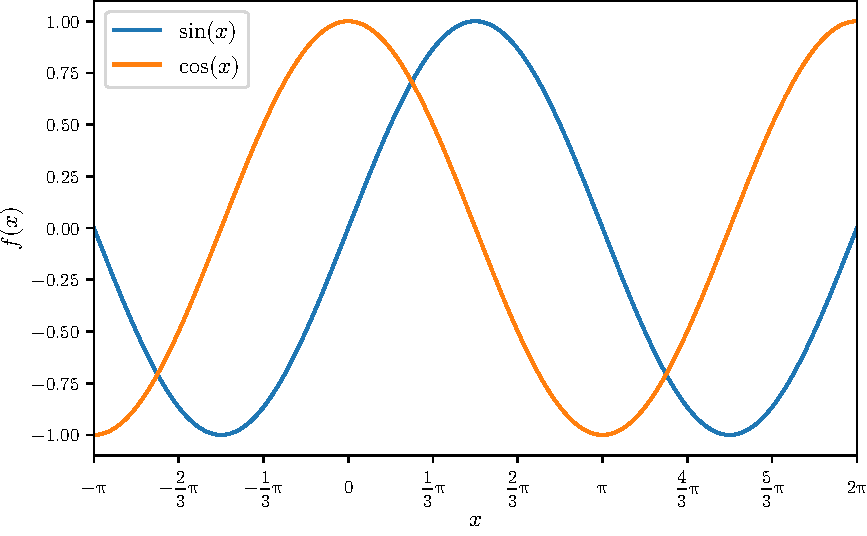
\includegraphics[scale=1]{plot1.pdf}
  \caption{Ein schöner Plot.}
  \label{fig:plot1}
\end{figure}
\blindtext

\section*{Aufgabe 2}

Abbildung~\ref{fig:subfigs} enthält zwei schöne Plots.
Wobei Abbildung~\ref{fig:plot2} der schönste aller Plots ist.

\begin{figure}%
  \begin{subfigure}{0.475\textwidth}%
    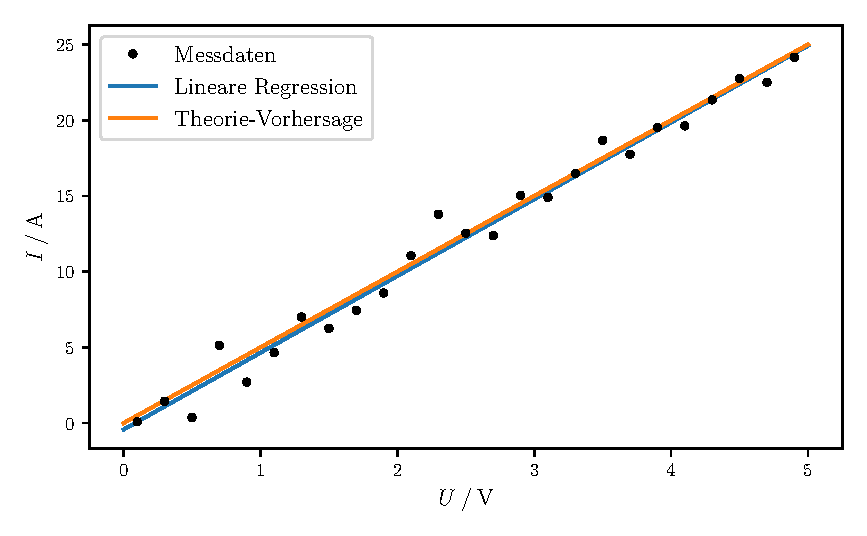
\includegraphics[width=\textwidth]{plot2.pdf}%
    \caption{Schöner Plot 2.}%
    \label{fig:plot2}%
  \end{subfigure}%
  \hfill%
  \begin{subfigure}{0.475\textwidth}%
    \centering%
    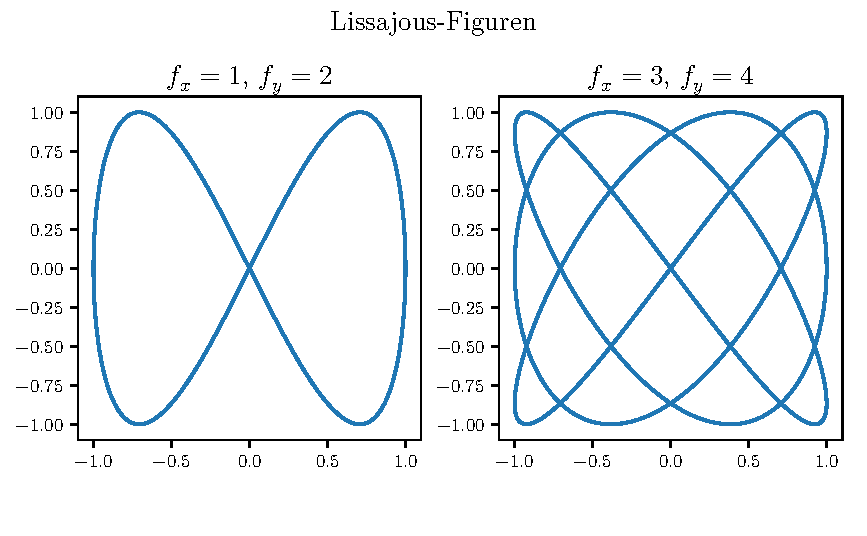
\includegraphics[width=\textwidth]{plot3.pdf}%
    \caption{Schöner Plot 3.}%
    \label{fig:plot3}%
  \end{subfigure}%
  \caption{%
    Zwei schöne Plots, Abbildung \subref{fig:plot2} und Abbildung \subref{fig:plot3}.
    Um die Breite dieser Caption zu demonstrieren, muss man sie noch viel länger machen.
    So langsam sollte es ausreichen.
    Aber die Schriftgröße und auch die Plots an sich sind zu klein.
    Nicht einfach Plots herunterskalieren!
  }\label{fig:subfigs}%
\end{figure}

\end{document}
